\documentclass[12pt]{report}
\usepackage{geometry}
\geometry{hmargin=2cm,vmargin=1.5cm}

\usepackage{hyperref}
\usepackage[T1]{fontenc}
\usepackage[utf8]{inputenc}
\usepackage[francais]{babel}

\usepackage{graphicx}

\title{Rapport de stage \\
Licence Informatique 3\up{ème} année}
\author{stagiaire : Athman Mekhzoumi\\
tuteur : Olivier Baudon} 

\begin{document}
\newpage
\maketitle
\tableofcontents
\newpage

\chapter{A modifier}

\section{Introduction}

Dans cette partie, nous allons présenter le thème du stage, les prérequis exigés, le travail demandé et dans quel contexte ce sujet a été posé.

\subsection{Sujet du stage}

Le sujet du stage est \textit{Publier une bibliothèque sur les graphes et la compléter}, une version beta de la bibliothèque était déjà implémenté avant le début du stage, les taches principales était de compléter le code là ou il y manquait, améliorer le code en s'inspirant des nouvelles version du langage \textit{java} et aussi documenter ansi que commenter la bibliothèque.
\newline Des connaissance en "Programmation orienté objet" et en "Théorie des graphes" m'étais nécessaire pour comprendre la conception et l'implémentation de la bibliothèque, heureusement pour j'avais déjà aqcuis les notions de base sur ces deux domaines au cours de mes études universitaires dans mon pays natale, mais cela ne m'été pas suffisant car il me fallait des connaissances plus profondes, alors j'ai lu quelques cours en ligne et codé programmes avant le début du stage pour étre au niveau éxigé. 

\subsection{Le contexte du stage}

Ce stage rentre dans le cadre du cycle licence, c'est stage obligatoire de 4 semaines minimum, il resprésente l'élément pédagogique 4TTVP18U et il fait partie du semèstre 6 du parcours informatique, l'obtention de ce stage été faite avec une candidature spontané adressé au Maître de Conférences Mr BAUDON Olivier qui fait partie de l'équipe des chercheurs du LaBRI.

\newpage
\section{Déroulement du stage}

Dans cette partie nous allons parler du travaille fait par l'étudiant, des compétences qui ont été mobilisé pour le réaliser ansi que les connaissances et compétences acquis et métrisés.

\subsection{première semaine}

\subsubsection{Les classes abstraites et les interfaces}

Une classe est définie comme abstraite avec le mot clé \textbf{abstract}, Les classes abstraites sont à utiliser lorsqu'une classe mère ne doit pas être instanciée, cette dernière peux t'avoir ce qu'on appelle une méthode abstraite qui est caractérisé par le fait qu'elle n'a pas de corps, comme elle peux t'avoir des méthodes normales, par contre si une classe contient une méthode abstraite, cette classe doit alors être déclarée abstraite.\newline
Une interface n'est q'une classe abstraite à 100\%, ce qui signifie aucune méthode d'une interface n'a de corps, elle sert à définir un supertype et à utiliser le polymorphisme, pour implémenter dans une classe il faut utiliser le mots clé \textbf{implements}, et on peut implémenter autant qu'on veux dans la même classe, pour que cela soit fait correctement il faut redéfinir toutes les méthodes de l'interface (ou des interfaces) dans la classe concerné.

\subsubsection{Les exceptions}
Lorsqu'un événement que la JVM ne sait pas gérer apparaît, une exception est levée (exemple : division par zéro). une exception correspond donc à une erreur, la superclasse qui gère les exceptions s'appelle \textbf{Exception}. C'est possible aussi de créer une classe d'exception personnalisée qui génère ce que le programmeur considère comme exception mais peux être pas par le JVM, pour y procéder il faut lui hériter de la classe Exception.\newline
L'instruction qui permet de capturer des exceptions est le bloc \textbf{try{…}catch{}}, si une exception est levée dans le bloc try, les instructions figurant dans le bloc catch seront exécutées pour autant que celui-ci capture la bonne exception levée. On peut aussi prévenir la JVM qu'une méthode est risque de générer une exeption grâce au mot clé \textbf{throws}. Une instanciation d'une exeception est lancée par le biais de l'instruction \textbf{throw}.

\subsubsection{Les varargs}
Les varargs pemettent de passer un nombre variable d’arguments à une méthode (pourvu qu’ils soient tous du type déclaré dans la signature de la méthode), sans créer explicitement de tableau, en revanche, dans le corps de la méthode, la variable var-arg est considéré comme un banal tableau et peut donc être parcourue par un « foreach », fournir sa taille avec la propriété length.
Il y a toutefois deux petites limitations à cette syntaxe :
\begin{itemize}
\item Il ne peut y avoir qu’un seul var-arg par signature de méthode.
\item Le var-arg doit toujours être le dernier paramètre.
\end{itemize}

\newpage
\subsection{Deuxième semaine}

\subsubsection{Les collection}
Les collection permet de stocker un nombre variable d'objets, il y a principalement trois types de collection : \textbf{List} et \textbf{Set} qui hérite de l'interface Collection et aussi le type \textbf{Map}. chaque type a ses avantages et ses inconvénients et fournies des fonctionnalités propre à lui.\newline
Voici quelques différences les différents types de collections:
\begin{itemize}
\item Les Collection stockent des objets alors que les Map stockent un couple (clé-valeur).
\item Si on insére fréquemment des données en milieu de liste, \textbf{LinkedList} est plus aprioprié.
\item Si on veut rechercher ou accéder à une valeur via une clé de recherche, vaut mieux opter pour une collection de type \textbf{Map}.
\item Si on veut traiter une grande quantité de données, le type \textbf{Set} convient le plus.
\end{itemize}

\subsubsection{La généricité}
La généricité est un concept très utile pour développer des objets travaillant avec plusieurs types de données, ça nous fait gagné du temps au lieu de développer des classes qui traite de façon identique des données de type différent.\newline
On peut utiliser la généricité sur les objets servant à gérer des collections, et avec l'outil \textbf{wildcard (?)} on indiquer que n'importe quel type peut être traité, mais cela revient à rendre ladite collection en lecture seule ce qui peux être désavantagant. 

\subsubsection{Git}
Pour Facilité la communication et entre le stagière et l'encadrant pendant tout le stage, même les weekend, la platforme github a été utiliser par pour sauvegader les changements fait sur la bibliothèque et aussi pour encadrer et guider le stagiere au fure et à mesure de son aprentissage.

~\\
\subsection{Troisième semaine}

\subsubsection{Diagramme UML}

La modélisation UML permet de vulgariser les aspects liés à la conception et à l’architecture, propres au logiciel (dans ce cas la bibliothèque), au client (dans ce cas les utilisateurs de cette derniere). Aussi, elle apporte une compréhension rapide du programme à d’autres développeurs externes en cas de reprise du logiciel et facilite sa maintenance. \newline
Pour ce projet j'ai utilisés \textbf{ObjectAid UML Explorer} qui est un outil de visualisation de code souple et léger pour l'IDE Eclipse. Il affiche le code source Java et les bibliothèques dans des diagrammes de classes et de séquences UML dynamiques qui se mettent automatiquement à jour lorsque mon code change.
La figure suivante représante les diagrammes UML obtenu à partir d'ObjectAid et en précisant les paramètres souhaités :

\begin{center}
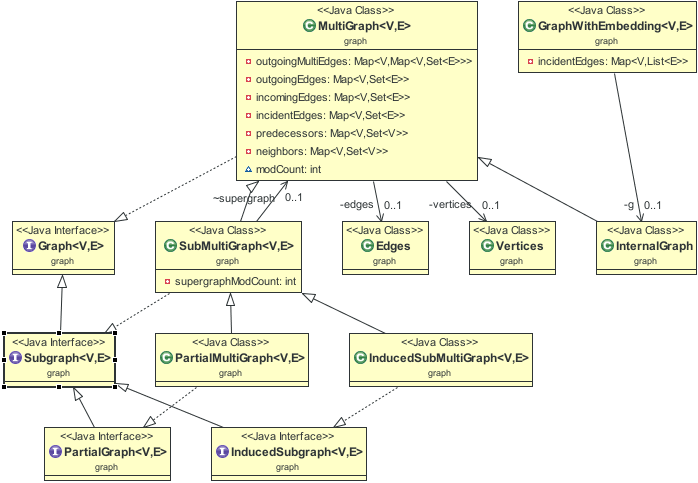
\includegraphics[width=1\textwidth]{DiagUMLPartie1.png}
\caption{\label{fig:DiagUMLPartie1}
~\\
~\\
~\\
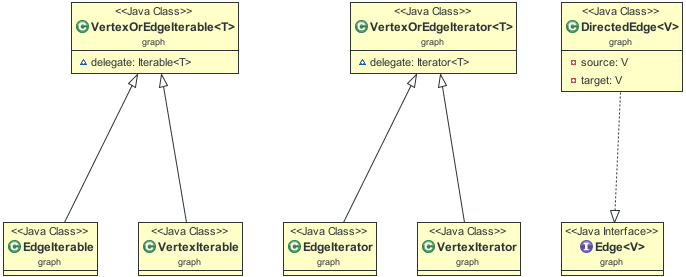
\includegraphics[width=1\textwidth]{DiagUMLPartie2.png}
\caption{\label{fig:DiagUMLPartie2}\newline Figure 1: \textit{Diagrammes UML du package "graphe" }}
\end{center}

\newpage
\subsubsection{Classe interne, locale et anonyme}

Une classe interne est déclarée à l'intérieur d'une autre classe, Elle peut donc accéder aux membres de la classe externe. Il y'as deux models pricipales de cette dernière, Les classe internes statiques qui ne peuvent accéder qu'aux membres statiques de leurs classes englobantes respectives, Les classes internes non statiques qui peuvent accéder aux membres statiques de leurs classes ainsi qu'aux membres des objets respectives qui les a créées.\newline

Une classe interne définie dans un bloc est une classe interne dont la portée est limitée au bloc : c’est une classe interne locale. Une classe locale ne peut pas être static. Une classe locale peut accéder aux attributs de la classe englobante ainsi qu'aux paramètres et variable locales de la méthode où elle est définie, à condition que ceux-ci soit spécifiés final.\newline 

Il est possible de définir une classe interne, sans lui donner de nom par dérivation d’un super classe, ou par implémentation d’une interface, c'est ce qu'on appel une classe anonyme. Elles ont utiles lorsqu'on a besoin de déclarer une classe pour l'utilisé une seul fois.


\subsubsection{Corretion des warnings}

Au début du stage la bibliothèque contenait multiples warning, pour toutes sorte de disfonctionnement ou de prolème eventuelle il fait retiré ces warnings. Pour cela chaque warning a été traité individuellement selon le problème qui le génère. Pour procéder a cette opération j'ai eu recours a deux solutions : les solutions proposés sur internet et l'utilitaire de réparation des warnings intégré à l'IDE ecplise.
~\\

\subsection{Quatrième semaine}
\subsubsection{Optimisation du code}
\subsubsection{Lambda expression}
\subsubsection{Entête et licence}

\section{Bilan du stage}

\newpage
\section{Référence}
\begin{verbatim}
https://openclassrooms.com/courses/apprenez-a-programmer-en-java/
les-classes-abstraites-et-les-interfaces

https://openclassrooms.com/courses/apprenez-a-programmer-en-java/
les-exceptions

http://thecodersbreakfast.net/index.php?post/2008/07/23/77-java-les-var-args

https://openclassrooms.com/courses/apprenez-a-programmer-en-java/
les-collections-d-objets

http://objectaid.com/

http://imss-www.upmf-grenoble.fr/prevert/Prog/Java/CoursJava/classes3.html
\end{verbatim}

\end{document}
